\section{Suffix array construction}
A suffix array is a permutation of string positions which lexicographically sorts the suffixes of the string starting at that position.
It is an influential data structure with many applications in efficient string algorithms solving problems such as exact pattern matching, repeat finding, maximum exact match (MEM) finding, document retrieval and many more.

There exist several algorithms for suffix array construction in linear time \cite{skew2003karkkainen,sais2009nong,saoverview2007puglisi} with several practical implementations \cite{louza2017inducing,libdivsufsort}.
Despite their linear time complexity, these algorithms become bottlenecks in some applications because of their linear space complexity.
This observation is especially relevant in pangenomics, where the datasets often do not fit in the computer memory.

Here, we show another crucial advantage of prefix-free graphs.
Although they do not offer any improvement of theoretical guarantees in the worst case, in practice, they often represent the pangenome in a substantially smaller space and allow us to generate the suffix array values one by one, possibly using the values directly in subsequential computation or storing them in compressed form.
This iteration can be done without ever expanding the pangenome to its textual representation in space proportional to the sum of segment lengths and the sum of path lengths.

\subsection{Iterator preparation}
To prepare the iterator of a suffix array of the pangenome from a prefix-free graph, we need to create several data structures.
First, we concatenate all the segments into a single string using a separator $\texttt{\#}$ and append a sentinel $\texttt{\$}$.
We will call this concatenation \emph{segment join}.
An example of a segment join is in Figure \ref{fig:ids_and_positions}.

Next, we calculate the segment join's suffix array and the longest common prefix array \cite{landau2001linear,manzini2004two}.
For both of these arrays, there exist algorithms with linear time and space complexity which we can use.
We note that these linear complexities are proportional to the length of the segment join, which is usually much smaller than the original pangenome.

Next, for each suffix of the segment join, we need to calculate the corresponding segment ID and position values.
The value segment ID represents in what segment the current suffix starts, and the value segment position represents at what position in that particular segment the current suffix starts.
These arrays can be computed using an inverse permutation of a suffix array $\texttt{ISA}$ (Equation \ref{eq:isa}) of a segment join in linear time.

\begin{equation}
    \label{eq:isa}
    \texttt{ISA}[\texttt{SA}[i]] = i
\end{equation}

To illustrate the procedure, consider the segment join of our running example from Figure \ref{fig:ids_and_positions}.
Each position of the join can be assigned a segment ID and a position in the current segment by linearly scanning the segment join and incrementing the ID and position accordingly.
Then, applying the ISA to these arrays changes the order of computed values in correspondence to the sorted suffixes.
The resulting suffix array $\texttt{SA}$, longest common prefix array $\texttt{LCP}$, segment ID array $\texttt{ID}$ and segment positions array $\texttt{pos}$ are stored in a \emph{suffix table} as shown in Table \ref{tab:suffix}.

\begin{figure}
    \centering
    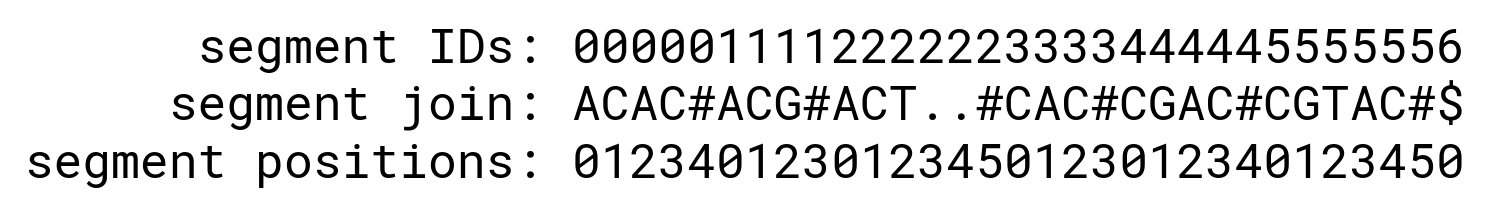
\includegraphics[width=\linewidth]{images/ids_and_positions.png}
    \caption{
    Segment join of segments from the running example, corresponding segment IDs, and positions. Permuting IDs and positions according to the \texttt{ISA} results in the segment ID array \texttt{ID} and the segment position array \texttt{pos} shown in Table \ref{tab:suffix}. \label{fig:ids_and_positions}
    }
\end{figure}

\begin{table*}
    \caption{
    Suffix table with the suffix array \texttt{SA}, longest common prefix array \texttt{LCP}, segment ID array \texttt{ID} and segment positions array \texttt{pos} of the running example. Suffixes of segment join from position \texttt{SA}[i] added for easier interpretation. Darker colours represent the suffix of the current segment. \label{tab:suffix}
    }
    \begin{tabular}{rrrrrl}
        \toprule
        i & \texttt{SA}[i] & \texttt{LCP}[i] & \texttt{ID}[i] & \texttt{pos}[i] & segment join[\texttt{SA}[i]..] \\
        \midrule
         0  & 30 & -1 & 6 & 0 & \texttt{\textcolor{gray}{\$}}                                     \\
         1  & 29 &  0 & 5 & 5 & \texttt{\textcolor{gray}{\#\$}}                                   \\
         2  &  4 &  1 & 0 & 4 & \texttt{\textcolor{gray}{\#ACG\#ACT..\#CAC\#CGAC\#CGTAC\#\$}}     \\
         3  &  8 &  3 & 1 & 3 & \texttt{\textcolor{gray}{\#ACT..\#CAC\#CGAC\#CGTAC\#\$}}          \\
         4  & 14 &  1 & 2 & 5 & \texttt{\textcolor{gray}{\#CAC\#CGAC\#CGTAC\#\$}}                 \\
         5  & 18 &  2 & 3 & 3 & \texttt{\textcolor{gray}{\#CGAC\#CGTAC\#\$}}                      \\
         6  & 23 &  3 & 4 & 4 & \texttt{\textcolor{gray}{\#CGTAC\#\$}}                            \\
         7  & 13 &  0 & 2 & 4 & \texttt{.\textcolor{gray}{\#CAC\#CGAC\#CGTAC\#\$}}                \\
         8  & 12 &  1 & 2 & 3 & \texttt{..\textcolor{gray}{\#CAC\#CGAC\#CGTAC\#\$}}               \\
         9  & 27 &  0 & 5 & 3 & \texttt{AC\textcolor{gray}{\#\$}}                                 \\
        10  &  2 &  3 & 0 & 2 & \texttt{AC\textcolor{gray}{\#ACG\#ACT..\#CAC\#CGAC\#CGTAC\#\$}}   \\
        11  & 16 &  3 & 3 & 1 & \texttt{AC\textcolor{gray}{\#CGAC\#CGTAC\#\$}}                    \\
        12  & 21 &  5 & 4 & 2 & \texttt{AC\textcolor{gray}{\#CGTAC\#\$}}                          \\
        13  &  0 &  2 & 0 & 0 & \texttt{ACAC\textcolor{gray}{\#ACG\#ACT..\#CAC\#CGAC\#CGTAC\#\$}} \\
        14  &  5 &  2 & 1 & 0 & \texttt{ACG\textcolor{gray}{\#ACT..\#CAC\#CGAC\#CGTAC\#\$}}       \\
        15  &  9 &  2 & 2 & 0 & \texttt{ACT..\textcolor{gray}{\#CAC\#CGAC\#CGTAC\#\$}}            \\
        16  & 28 &  0 & 5 & 4 & \texttt{C\textcolor{gray}{\#\$}}                                  \\
        17  &  3 &  2 & 0 & 3 & \texttt{C\textcolor{gray}{\#ACG\#ACT..\#CAC\#CGAC\#CGTAC\#\$}}    \\
        18  & 17 &  2 & 3 & 2 & \texttt{C\textcolor{gray}{\#CGAC\#CGTAC\#\$}}                     \\
        19  & 22 &  4 & 4 & 3 & \texttt{C\textcolor{gray}{\#CGTAC\#\$}}                           \\
        20  &  1 &  1 & 0 & 1 & \texttt{CAC\textcolor{gray}{\#ACG\#ACT..\#CAC\#CGAC\#CGTAC\#\$}}  \\
        21  & 15 &  4 & 3 & 0 & \texttt{CAC\textcolor{gray}{\#CGAC\#CGTAC\#\$}}                   \\
        22  &  6 &  1 & 1 & 1 & \texttt{CG\textcolor{gray}{\#ACT..\#CAC\#CGAC\#CGTAC\#\$}}        \\
        23  & 19 &  2 & 4 & 0 & \texttt{CGAC\textcolor{gray}{\#CGTAC\#\$}}                        \\
        24  & 24 &  2 & 5 & 0 & \texttt{CGTAC\textcolor{gray}{\#\$}}                              \\
        25  & 10 &  1 & 2 & 1 & \texttt{CT..\textcolor{gray}{\#CAC\#CGAC\#CGTAC\#\$}}             \\
        26  &  7 &  0 & 1 & 2 & \texttt{G\textcolor{gray}{\#ACT..\#CAC\#CGAC\#CGTAC\#\$}}         \\
        27  & 20 &  1 & 4 & 1 & \texttt{GAC\textcolor{gray}{\#CGTAC\#\$}}                         \\
        28  & 25 &  1 & 5 & 1 & \texttt{GTAC\textcolor{gray}{\#\$}}                               \\
        29  & 11 &  0 & 2 & 2 & \texttt{T..\textcolor{gray}{\#CAC\#CGAC\#CGTAC\#\$}}              \\
        30  & 26 &  1 & 5 & 2 & \texttt{TAC\textcolor{gray}{\#\$}}                                \\
        \bottomrule
    \end{tabular}
\end{table*}




\begin{table}
    \caption{
    Segment table containing an id, length, starting positions in the concatenated pangenome and ranks of the right contexts of these positions for each segment. \label{tab:segment}}
    \begin{tabular}{rrll}
        \toprule
        id & length & starts & right context ranks \\
        \midrule
        0 & 4 & 9           & 9         \\
        1 & 3 & 15, 1       & 13, 14    \\
        2 & 5 & 18, 5, 11   & 1, 2, 3   \\
        3 & 3 & 8, 14, 0    & 4, 5, 6   \\
        4 & 4 & 16          & 7         \\
        5 & 5 & 2           & 8         \\
        \bottomrule
    \end{tabular}
\end{table}



In the suffix table, one row can represent multiple positions of the pangenome.
% These positions can be represented as a single integer coresponding to index in the concatenated representation of a pangenome.
To identify these positions, we store some additional information in a \emph{segment table}.
For each segment of the prefix-free graph, we store its length, starting positions in the concatenated pangenome and ranks of the right contexts of these positions.
To calculate the starting positions and the ranks of the right contexts, we use a \emph{path join}.
Similarly to segment join, a path join is a concatenation with delimiters $\texttt{\#}$ and sentinel $\texttt{\$}$, but now constructed by concatenating the paths.
An example of a path join for our running example is in Figure \ref{fig:path_join}.
Then, starting positions can be calculated by cumulatively summing the lengths
of the segments in path join and subtracting the overlaps.

The computation of ranks is more involved.
It uses the normalized form of prefix-free graphs since it relies on a lexicographically smaller ID in a path representing a lexicographically smaller segment.
We construct the suffix array of the path join and find its inverse permutation $\texttt{ISA}$.
$\texttt{ISA}$ gives us ranks for each position in the path join.
To determine the rank of the right context for position $i$, we take
the value of $\texttt{ISA}[i+1]$.
Finally, we store the starts and ranks sorted by the rank values in the segment table as shown in Table \ref{tab:segment}.

\begin{figure}
    \centering
    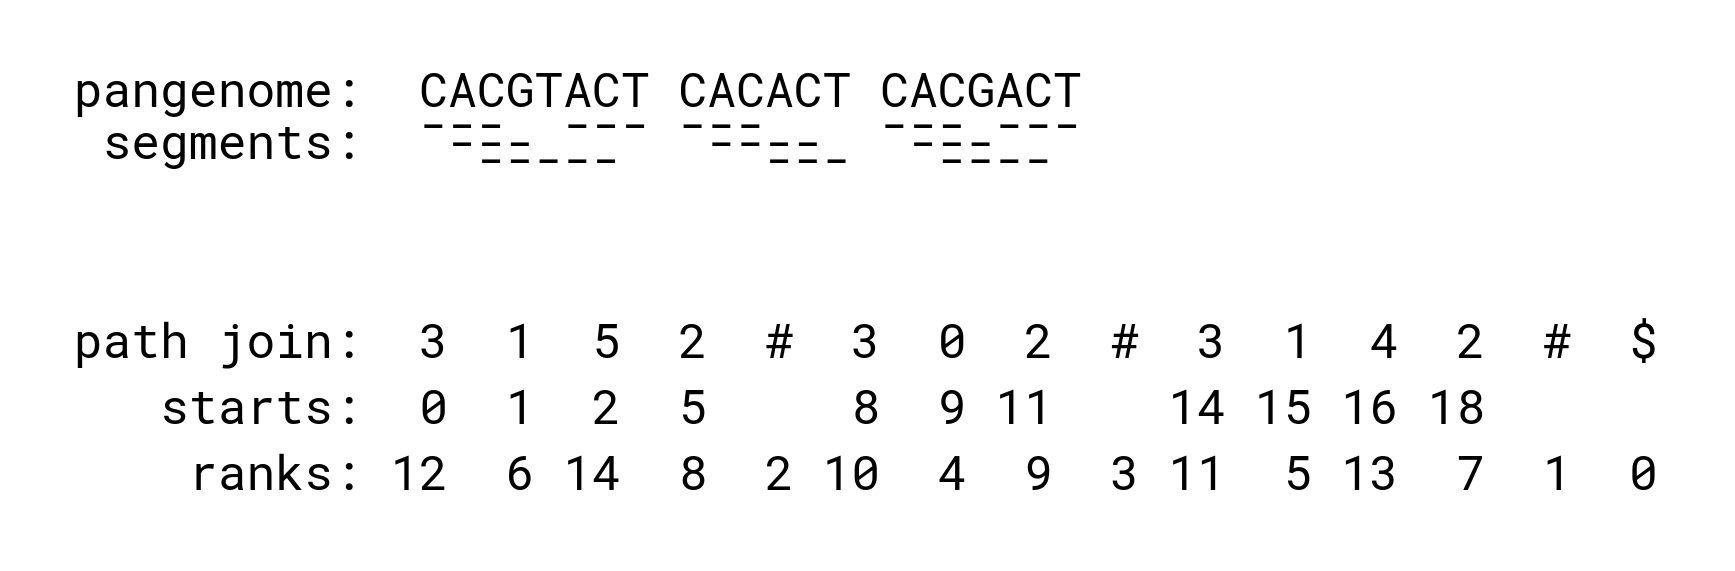
\includegraphics[width=\linewidth]{images/path_join.png} %% TODO: change this
    \caption{
    Path join of paths from the running example and the corresponding starts and ranks. The concatenated pangenome and segments are shown above to clarify the meaning of the start values. \label{fig:path_join}
    }
\end{figure}

\subsection{Iteration}
With the previous tables stored in memory, we have all the necessary ingredients to generate the suffix array value by value.

Each row in the suffix table represents a suffix of a particular segment.
There are four cases of what the first position of these suffixes can represent within the segments:
\begin{itemize}
    \item the sentinel $\texttt{\$}$
    \item a separator $\texttt{\#}$
    \item a position within the last $k$ characters of a segment
    \item a position outside the last $k$ characters, separator and sentinel
\end{itemize}

Since the pangenome has no corresponding position for the sentinel or separator characters, we can skip the first rows representing them.

In the third case, the position is inside the trigger word or the sentinels appended during the graph construction.
The positions inside the trigger words are represented twice in the suffix table, once at the end of a segment and a second time at the beginning of the following segment in the pangenome.
These ending positions can violate the prefix-free property of the segment suffixes and, therefore, can be sorted incorrectly.
Skipping through these positions ensures the prefix-free property for the rest of the suffixes and also avoids double reporting.
Therefore, if the length of a current segment suffix is smaller or equal to the size of the trigger words $k$, we skip the row as in the previous cases.
This choice also plays nicely with the previous choice of appending $k$ sentinels during the construction of a prefix-free graph, as these positions will not get reported either.

Finally, in the last case, we report the suffix array values.
The suffix table can be partitioned into blocks of the same segment suffixes.
For example, consider rows 20 and 21, which form a single block.
All other blocks in the running example consist of single rows; therefore, we call them singletons.

This partitioning leads to three cases:
\begin{itemize}
    \item a singleton block with segment suffix occurring only once in the whole pangenome
    \item a singleton block with segment suffix occurring several times in the pangenome
    \item a non-singleton block
\end{itemize}

In the first case, we must report only a single suffix array value.
Given the row index $i$, this value can be calculated with Equation \ref{eq:sa_value}.

\begin{equation}
    \label{eq:sa_value}
    \texttt{SA value} = \texttt{starts}[\texttt{ID}[i]] + \texttt{pos}[i]
\end{equation}

As an example, consider the row $13$ in Table \ref{tab:suffix}, the first row yielding a SA value.
Its segment ID is $0$, and from Table \ref{tab:segment}, we see only one occurrence of segment $0$ with starting position $9$ in the pangenome.
The offset from the start of a segment $\texttt{pos}[13]$ is $0$.
Summing these two values, we get the first value of a suffix array $9 + 0 = 9$ corresponding to the lexicographically smallest suffix of a concatenated pangenome $P[9..] = \texttt{ACACT}$.

The second, slightly more complex case is a singleton block representing a segment suffix with several occurrences in the pangenome.
In this case, we must report as many suffix array values as the number of occurrences.
Because the starting segment positions in the segment table are sorted based on their right context rank, we can iterate through these starting positions and apply Equation \ref{eq:sa_value} to each of them.

As an example, consider the row $14$ in Table \ref{tab:suffix}.
This suffix occurs twice in the pangenome in segments starting at positions $15$ and $1$.
Since the offset from the start of a segment $\texttt{pos}[14]$ is $0$, we report a suffix array values $15 + 0 = 15$ and $1 + 0 = 1$, corresponding to the suffixes $P[15..] = \texttt{ACGACT}$ and $P[1..] = \texttt{ACGTACT}$.

In the last case, we have a non-singleton block representing suffixes of several segments, possibly with multiple occurrences.
These suffixes represent identical substrings in the original pangenome.
Here, we report a suffix array value for each of the substrings.
To identify the first value, we must find the starting position with the smallest right context rank.
Because the ranks are sorted, this procedure is similar to the merging phase of a merge sort.
Therefore, to iterate through all suffix array values in the block, we always identify the segment start with the next smallest right context rank and apply Equation \ref{eq:sa_value} to this segment start.

As an example, consider the block of rows $[20..21]$ in Table \ref{tab:suffix}.
The relevant segment IDs are $0$ and $3$, with segment starts at positions $9$, $8$, $14$ and $0$.
The right context ranks from smallest to highest are $4, 5, 6, 9$ with the corresponding segment starts $8, 14, 0, 9$.
Applying Equation \ref{eq:sa_value} to these segment starts yields a suffix array values $8 + 0 = 8$, $14 + 0 = 14$, $0 + 0 = 0$ and $9 + 1 = 10$, representing pangenome suffixes $P[8..] = \texttt{CACACT}$, $P[14..] = \texttt{CACGACT}$, $P[0..] = \texttt{CACGTACT}$, and $P[10..] = \texttt{CACT}$.

